Teoria węzłów to gałąź topologii,
która powstała z~inspiracji węzłami,
jakie pojawiają się w~codziennym życiu: przy wiązaniu butów albo cumowaniu statków.
Zajmuje się ona badaniem przede wszystkim węzłów,
czyli pewnych włożeń okręgu $S^1$ w~trójwymiarową przestrzeń euklidesową $\R^3$ lub sferę $S^3$,
ale także splotów (zaplątanych w~sobie węzłów), warkoczy, supłów oraz podobnych obiektów.
Matematyczne węzły różnią się tym od zwykłych, że ich końce są ze sobą połączone.

Oto kilka przykładów.
Węzeł (a) nazywamy niewęzłem, jest to kalka angielskiego \emph{unknot}.
Następne w~kolejce widoczne są trójlistnik (b,~\emph{trefoil}), ósemka (c,~\emph{figure-eight}), pięciolistnik (d,~\emph{cinquefoil}) oraz słynna para Perko (e,~f~wg oryginalnej numeracji Rolfsena).
Pod diagramami umieściliśmy notację Alexandera-Briggsa, jeszcze do niej wrócimy.

\begin{comment}
\begin{figure}[H]
    \centering
    \begin{minipage}[b]{.14\linewidth}
        \centering
        $\begin{tikzpicture}[baseline=-0.65ex, scale=0.5] \begin{knot}[clip width=5, end tolerance=1pt] \strand[semithick] (0,0) circle (\linewidth); \end{knot}
\end{tikzpicture}$
        \subcaption{}
    \end{minipage}
    \begin{minipage}[b]{.14\linewidth}
        \centering
        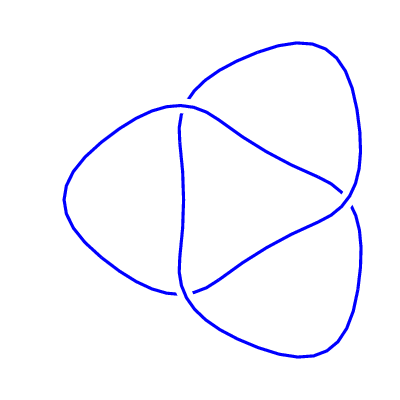
\includegraphics[width=\linewidth]{../data/3_1.png}
        \subcaption{$3_1$}
    \end{minipage}
    \begin{minipage}[b]{.14\linewidth}
        \centering
        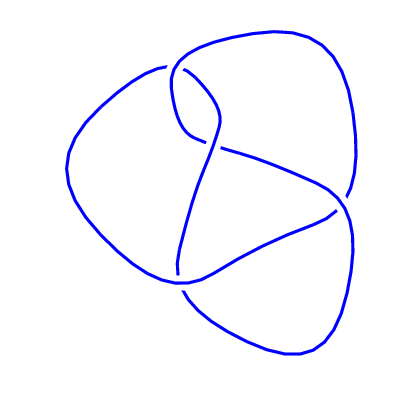
\includegraphics[width=\linewidth]{../data/4_1.png}
        \subcaption{$4_1$}
    \end{minipage}
    \begin{minipage}[b]{.14\linewidth}
        \centering
        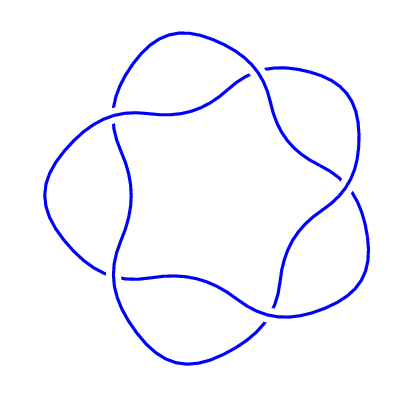
\includegraphics[width=\linewidth]{../data/5_1.png}
        \subcaption{$5_1$}
    \end{minipage}
    \begin{minipage}[b]{.14\linewidth}
        \centering
        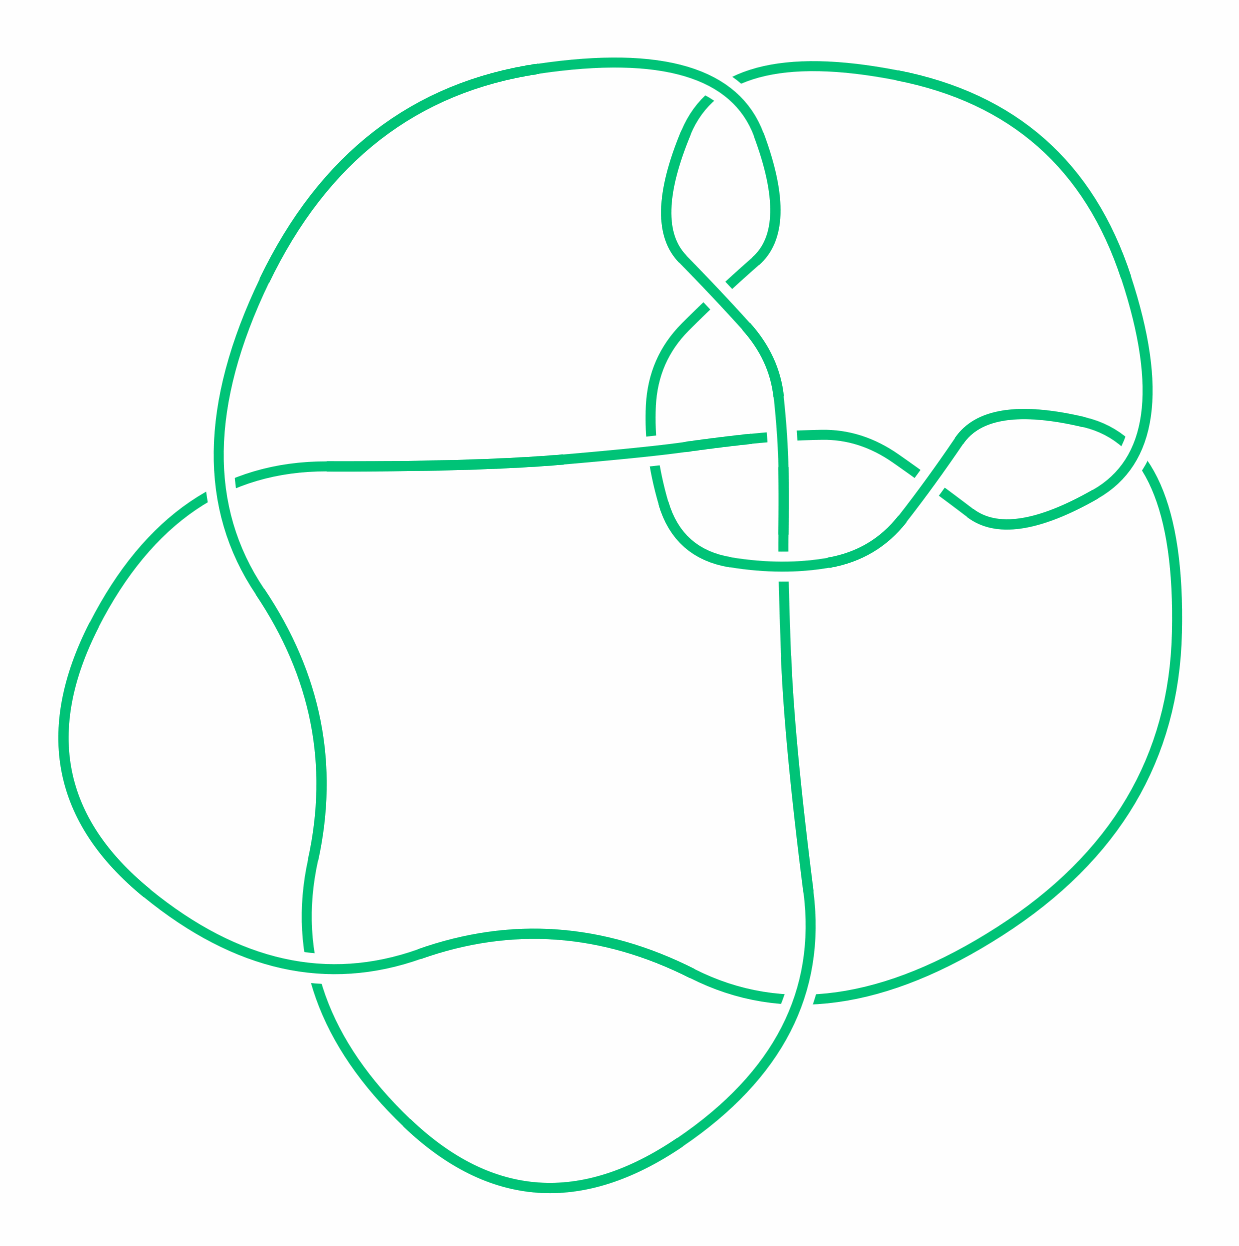
\includegraphics[width=\linewidth]{../data/perko1.png}
        \subcaption{$10_{161}$}
    \end{minipage}
    \begin{minipage}[b]{.14\linewidth}
        \centering
        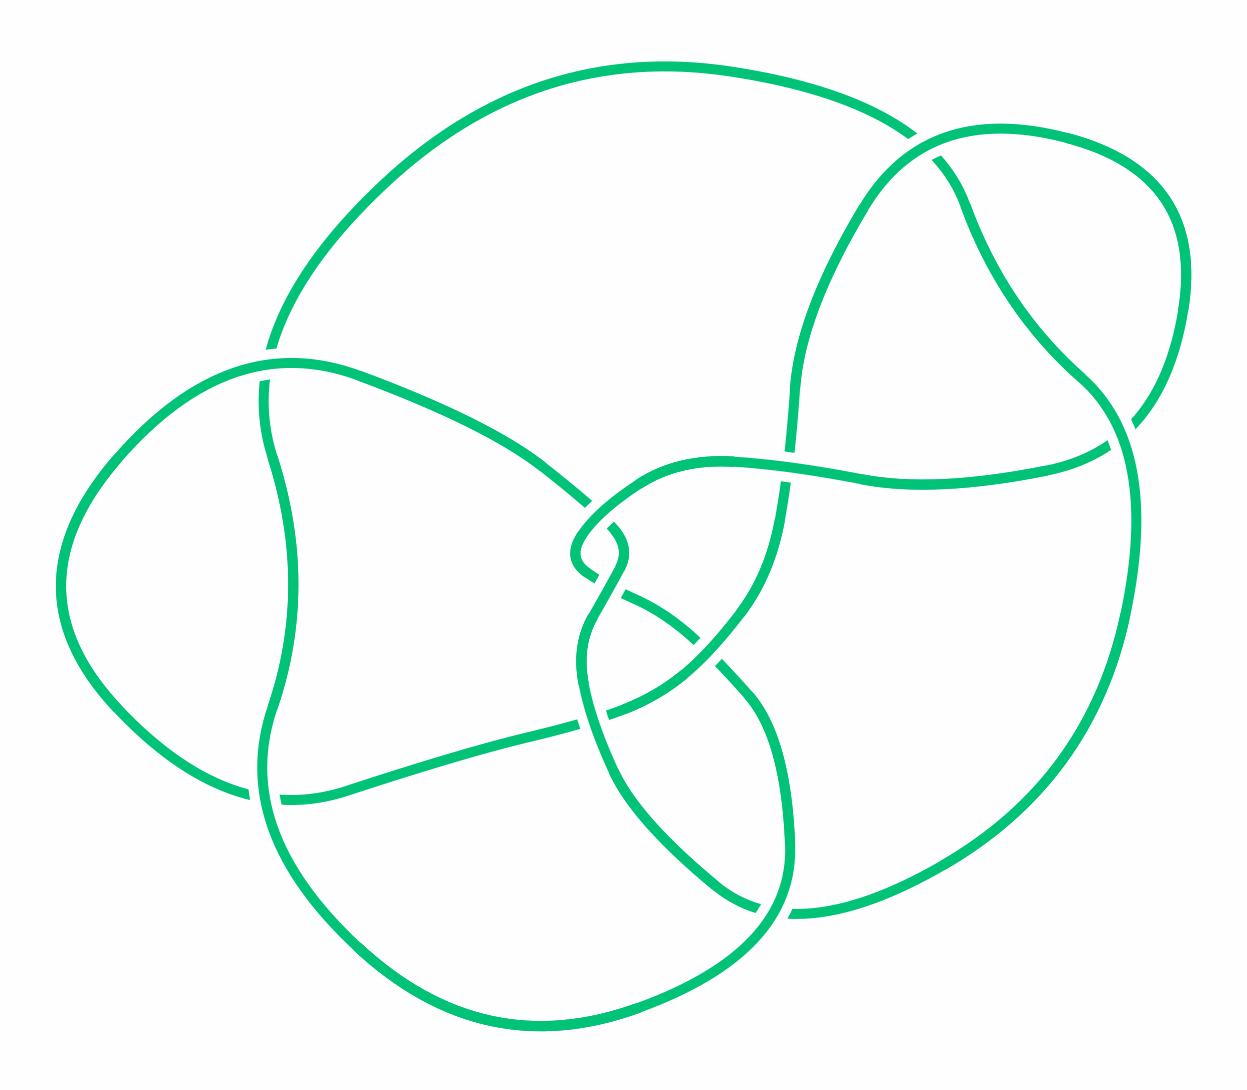
\includegraphics[width=\linewidth]{../data/perko2.png}
        \subcaption{$10_{162}$}
    \end{minipage}
\end{figure}
\end{comment}

Początkowo celem teorii węzłów była klasyfikacja wszystkich węzłów.
Od XIX wieku, kiedy teoria węzłów wyodrębniła się jako osobny dział matematyki,
zdążyliśmy skatalogować ponad sześć miliardów tych obiektów.
Pozornie tak samo wyglądające węzły mogą się od siebie różnić.
Do wykrywania tych subtelnych różnic używa się przede wszystkim niezmienników topologicznych takich jak grupy, wielomiany bądź liczby.
Poznamy je w~dalszych rozdziałach.

Matematycy uogólnili pojęcie węzła:
można rozpatrywać je w~wyższych wymiarach albo zastąpić okrąg inną przestrzenią topologiczną.
Będziemy starać się unikać tych uogólnień.

\section{Węzły i~sploty}
Największą różnicą między węzłami matematycznymi oraz tymi z~prawdziwego jest życia jest to, że te pierwsze nie mają luźnych końców.
Można przyjąć nieidealną, naiwną definicję:

\begin{definition}[węzeł]
    Ciągłe oraz różnowartościowe odwzorowanie $S^1 \to \R^3$ nazywamy węzłem.
\end{definition}

Niestety, dopuszcza ona patologiczne z~kombinatorycznego punktu widzenia węzły dzikie, jak ten z~rysunku \ref{wild_knot}:

\begin{comment}
\begin{figure}
    \centering
    \label{wild_knot}
    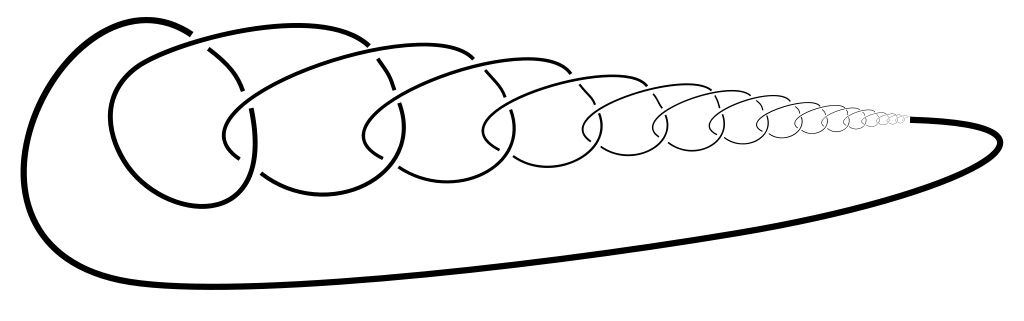
\includegraphics[width=0.5\linewidth]{wild_knot.png}
    \caption{Węzeł dziki}
\end{figure}
\end{comment}

Zastanówmy się, jakim formalizmem opisać manipulowanie fizycznym sznurkiem, by wykluczyć węzły dzikie z~naszych rozważań.
Nie można użyć izotopii (dwa węzły są izotopijne, jeśli istnieje ciągła funkcja $F \colon S^1 \times [0, 1] \to \R^3$ taka, że $F(-, 0)$ jest pierwszym, zaś $F(-,1)$ drugim węzłem), gdyż każdy węzeł jest izotopijny z punktem:

% TODO: Tu brakuje obrazka.

W podobny sposób moglibyśmy przekształcić dowolny węzeł w~niewęzeł.
Teoria, w~której wszystkie obiekty są takie same, nie jest zbyt ciekawa.
Zwykła izotopia nie oddaje dobrze tego, czym jest równoważność węzłów wykonanych z~prawdziwego sznurka.
Trzeba od niej wymagać dodatkowo, by była gładka albo lokalnie płaska.
Z twierdzenia o rozszerzaniu izotopii wynika, że można ją wtedy podnieść do izotopii otaczającej.
Ta ostatnia uwzględnia, jak węzeł leży w~przestrzeni i okazuje się być właściwym pojęciem równości dla teorii węzłów:

\begin{definition}[izotopia otaczająca]
    \label{def_ambient_isotopy}
    Niech $N, M$ będą rozmaitościami, zaś $K_1, K_2 \colon N \to M$ włożeniami.
    Ciągłe odwzorowanie $F \colon M \times [0,1] \to M$ spełniające następujące warunki:
    \begin{enumerate}
        \item funkcja $F(-, 0)$ jest odwzorowaniem tożsamościowym,
        \item każda z funkcji $F(-, t)$ jest homeomorfizmem,
        \item złożenie $F(-, 1)$ z pierwszym włożeniem $K_1$ daje drugie włożenie $K_2$
    \end{enumerate}
    nazywamy izotopią otaczającą przenoszącą $K_1$ na $K_2$.
\end{definition}

W topologii rozważa się włożenia dowolnych rozmaitości, nam wystarczy jeden szczególny przypadek $N = S^1$ oraz $M = \R^3$.
Intuicyjnie, funkcja $F$ zniekształca przestrzeń $\R^3$ tak, że w~chwili początkowej $t = 0$ widzimy pierwszy, zaś w~chwili końcowej $t = 1$ drugi węzeł.
Izotopia otaczająca nie pozwala na ściąganie zaplątanych fragmentów do punktu.

% TODO: Homeomorfizmy $F_t$ można zastąpić przez dyfeomorfizmy zachowujące orientację.

\begin{definition}[węzeł]
    \label{def:knot}
    \index{węzeł}
    Gładkie włożenie $S^1 \to \R^3$ otaczająco izotopijne z~zamkniętą łamaną bez samoprzecięć nazywamy węzłem poskromionym.
\end{definition}

Przez prawie całą książkę interesować nas będą jedynie węzły poskromione,
dlatego jeśli nie zaznaczono inaczej, przez węzeł rozumiemy węzeł poskromiony.
Istnieje jeszcze jedna, konkurencyjna definicja węzłów równoważnych:

\begin{proposition}
    \label{equivalent_knots_2}
    Dwa węzły są równoważne, gdy jeden z~nich jest obrazem drugiego przez zachowujący orientację homeomorfizm $\R^3 \to \R^3$.
\end{proposition}

Stwierdzenie to przestaje być prawdziwe po zastąpieniu przestrzeni $\R^m$ przez $S^m$.

\begin{proof}
    Podany niżej dowód pochodzi z~książki ,,Topology from the differentiable viewpoint'' Johna Milnora.
    Musimy pokazać, że dyfeomorfizm $f \colon \R^m \to \R^m$ jest gładko izotopijny z~identycznością.
    Translacje są izotopiami, więc bez straty ogólności zakładamy, że $f(0) = 0$.
    Pochodna $f$ w~zerze jest dana wzorem $\mathrm{d}f_0(x) = \lim_{t \to 0} f(tx) /t$,
    naturalną definicję izotopii $F \colon \R^m \times [0, 1] \to \R^m$ stanowi więc
    \[
        F(x, t) = \begin{cases}
            \mathrm{d}f_0(x) & t = 0 \\
            f(tx) / t & 0 < t \le 1
        \end{cases} .
    \]

    Funkcja $F$ jest gładka, gdyż na mocy lematu Hadamarda funkcja $f$ zapisuje się jako suma $x_1 g_1(x) + \ldots + x_mg_m(x)$, gdzie funkcje $g_i$ są gładkie, co jakoś kończy dowód.
\end{proof}

Formalnie węzły to pewne odwzorowania, więc prawidłowym sposobem na zapisanie, że są izotopijne (czyli dla nas: równe), jest $K_1 \simeq K_2$.
Ponieważ nie prowadzi to do problemów, będziemy jednak stosować zapis $K_1 = K_2$.
Jednocześnie często węzeł (jako odwzorowanie) nie będzie odróżniany od obrazu tego odwzorowania.

\begin{definition}[splot, ogniwo]
    \label{def_link}
    \index{splot}
    Sumę parami rozłącznych węzłów $K_1, K_2, \ldots, K_n$ nazywamy splotem.
    Składniki sumy nazywamy ogniwami.
\end{definition}

Przez analogię do węzłów mówimy, że dwa sploty są takie same, jeśli jeden jest obrazem drugiego przez zachowujący orientację homeomorfizm $\R^3 \to \R^3$.
W~takiej sytuacji obydwa sploty mają tyle samo ogniw.

\begin{example}
    \index{splot!Hopfa}
    Splot Hopfa to najprostszy splot nietrywialny, którym w~1931 r. zajmował się Heinz Hopf, topolog niemiecki, w~ramach badań nad tzw. rozwłóknieniem (Hopf fibration).
\end{example}

\begin{example}
    \index{splot!Whiteheada}
    Whitehead w~1934 odkrył kontrprzykład do nieudanego dowodu hipotezy Poincarego.
    Był nim splot o~dwóch składowych przedstawiony na poniższym rysunku.
\end{example}

\begin{comment}
    \begin{figure}[H]
        \begin{minipage}[b]{.48\linewidth}
            \centering
            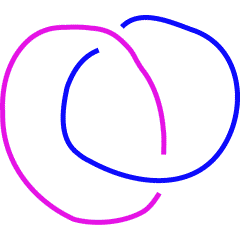
\includegraphics[width=0.5\linewidth]{../data/mixed/L2a1.png}
            \subcaption{splot Hopfa}
        \end{minipage}
        \begin{minipage}[b]{.48\linewidth}
            \centering
            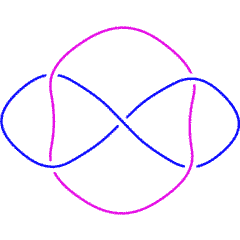
\includegraphics[width=0.5\linewidth]{../data/mixed/L5a1.png}
            \subcaption{splot Whiteheada}
        \end{minipage}
    \end{figure}
\end{comment}

Jeśli dwa węzły są równoważne, to ich dopełnienia są oczywiście homeomorficzne.
Pytanie o~prawdziwość implikacji odwrotnej jako pierwszy zadał najprawdopodobniej w~1908 roku Tietze (,,Über die topologischen Invarianten mehrdimensionaler Mannigfaltigkeiten'').
W roku 1987 pokazano, że istnieją co najwyżej dwa węzły o~zadanym dopełnieniu (\cite{culler87}).
Dwa lata później poznaliśmy pozytywną odpowiedź na pytanie Tietzego: każdy węzeł jest wyznaczony jednoznacznie przez swoje dopełnienie.

\begin{theorem}[Gordon, Luecke, 1989]
    \label{thm_gordon_luecke}
    \index{twierdzenie!Gordona-Lueckego}
    Poskromione węzły o~homeomorficznych (z zachowaniem orientacji) dopełnieniach są wzajemnie izotopijne.
\end{theorem}

\begin{proof}[Niedowód]
    Wynika to z~ogólniejszego stwierdzenia:
    nietrywialna chirurgia Dehna na węźle w~3-sferze nigdy nie daje 3-sfery.
    Pełny dowód zawiera praca \cite{gordon89}.
\end{proof}

Twierdzenie to zamienia problem lokalny (czy dwa węzły w kuli $S^3$ są równoważne?) w~problem globalny (czy dwie przestrzenie topologiczne są homeomorficzne?).
Whitehead w~pracy \cite{whitehead37} z~1937 roku podał nieskończenie wiele splotów, których dopełnienia wyglądają jak dopełnienia splotu Whiteheada.
Odpowiednik twierdzenia \ref{thm_gordon_luecke} dla splotów jest więc fałszywy.

Poniższa definicja nie jest nam jeszcze potrzebna, ale wygodnie przytoczyć ją już teraz.

\begin{definition}[rozszczepialność]
    \index{splot!rozszczepialny}
    Jeżeli splot $L$ można zanurzyć w przestrzeni $\R^3$ tak, że niektóre jego ogniwa będą leżeć nad pewną rozłączną ze splotem płaszczyzną, zaś pozostałe pod nią, to powiemy, że splot $L$ jest rozszczepialny.
\end{definition}

Liczbę nierozszczepialnych splotów, pierwszych lub złożonych, zebrano w tabeli.
Źródło: baza danych OEIS, ciąg \href{https://oeis.org/A086825}{A086825}.

\renewcommand*{\arraystretch}{1.4}
\footnotesize
\begin{longtable}{lccccccccc}
    \hline
    \textbf{skrzyżowania}  &  0  &  1  &  2  &  3  &  4  &  5  &  6   &  7   &  8   \\  \hline  \endhead
    sploty                 &  1  &  0  &  1  &  1  &  3  &  4  &  15  &  24  &  82  \\
    \hline
\end{longtable}
\normalsize

\section{Diagramy. Ruchy Reidemeistera}
Chociaż w~świetle definicji \ref{def:knot} węzły są pewnymi regularnymi podzbiorami przestrzeni $\R^3$,
z kombinatorycznego punktu widzenia wygodniej jest rysować je na płaszczyźnie.

\begin{definition}[orientacja]
    \index{splot!zorientowany}
    Węzeł, w~którym wybrano kierunek, w~którym należy się po nim poruszać, nazywamy zorientowanym.
    Splot nazywamy zorientowanym, jeśli wszystkie jego ogniwa traktowane jako węzły są zorientowane.
\end{definition}

\begin{definition} [diagram] \label{def_diagrams}
    \index{diagram}
    Cień to rzut węzła $K \subseteq \R^3$ na płaszczyznę.
    Cień razem z~informacją o~tym, jak przebiegają skrzyżowania i pozbawiony katastrof: potrójnych przecięć, stycznych czy dziobów nazywamy diagramem.
\end{definition}

% TODO: Narysować katastrofy

\begin{definition} [włókno]
    \index{włókno}
    Fragment diagramu, który biegnie między dwoma kolejnymi tunelami, czyli podskrzyżowaniami, nazywamy włóknem.
\end{definition}

\begin{definition} [nić]
    \index{nić}
    Fragment diagramu, który biegnie między dwoma kolejnymi skrzyżowaniami nazywamy nicią.
\end{definition}

Nici powstają z włókien przez rozcięcie ich przy każdym nadskrzyżowaniu.

\begin{proposition}
    Niech $K$ będzie węzłem.
    Zbiór diagramów jest otwarty i~gęsty w~zbiorze wszystkich rzutów.
\end{proposition}

\begin{proof}
    Rzut splotu na równoległe płaszczyzny jest taki sam, a te można sparametryzować prostymi przechodzącymi przez początek układu współrzędnych, które tworzą przestrzeń rzutową $\R \mathbb P^2$.
    Niech $S$ będzie zbiorem prostych, które dają złe rzuty.
    Wystarczy pokazać jego nigdziegęstość.
    Okazuje się, że $S$ jest też jednowymiarowy.
    (Dowód za \cite{crowell63}).
\end{proof}

Wynika stąd, że każdy węzeł ma wiele diagramów.
Mając dane dwa różne diagramy chcielibyśmy wiedzieć, czy reprezentują ten sam węzeł.
Na szczęście Reidemeister w latach 20. XX wieku podał proste kryterium rozstrzygające ten problem.
Najpierw zdefiniujmy trzy lokalne operacje na diagramach.

\begin{definition}[ruchy Reidemeistera]
    \index{ruchy!Reidemeistera}
    Trzy gatunki lokalnych deformacji diagramu splotu:
\begin{comment}
    \[
        \underbrace{\begin{tikzpicture}[baseline=-0.65ex,scale=0.1]
        \begin{knot}[clip width=5]
            \strand[thick] (-5, 10) to [in=left, out=down] (2, -5);
            \strand[thick] (5, 0) to [in=right, out=down] (2, -5);
            \strand[thick] (5, 0) to [in=right, out=up] (2, 5);
            \strand[thick] (-5, -10) to [in=left, out=up] (2, 5);
        \end{knot}
        \end{tikzpicture}
        \, \cong \,
        \begin{tikzpicture}[baseline=-0.65ex,scale=0.1]
        \begin{knot}[clip width=5]
            \strand[thick] (0,10) to (0,-10);
        \end{knot}
        \end{tikzpicture}}_{R_1}
        %%%
        \quad \quad \quad
        \underbrace{\begin{tikzpicture}[baseline=-0.65ex,scale=0.1]
        \begin{knot}[clip width=5]
            \strand[thick] (-5, 10) to [in=up, out=down] (5, 0);
            \strand[thick] (-5, -10) to [in=down, out=up] (5, 0);
            \strand[thick] (5, 10) to [in=up, out=down] (-5, 0);
            \strand[thick] (5, -10) to [in=down, out=up] (-5, 0);
        \end{knot}
        \end{tikzpicture}
        \, \cong \,
        \begin{tikzpicture}[baseline=-0.65ex,scale=0.1]
        \begin{knot}[clip width=5]
            \strand[thick] (-5, 10) to [in=up, out=down] (-2, 0);
            \strand[thick] (-5, -10) to [in=down, out=up] (-2, 0);
            \strand[thick] (5, 10) to [in=up, out=down] (2, 0);
            \strand[thick] (5, -10) to [in=down, out=up] (2, 0);
        \end{knot}
        \end{tikzpicture}}_{R_2}
        %%%
        \quad \quad \quad
        \underbrace{\begin{tikzpicture}[baseline=-0.65ex,scale=0.1]
        \begin{knot}[clip width=5, flip crossing/.list={1,2,3}]
            \strand[thick] (-10, -10) -- (10, 10);
            \strand[thick] (-10, 10) -- (10, -10);
            \strand[thick] (-10, 0) to [in=left, out=right] (0, 10);
            \strand[thick] (10, 0) to [in=right, out=left] (0, 10);
        \end{knot}
        \end{tikzpicture}
        \, \cong \,
        \begin{tikzpicture}[baseline=-0.65ex,scale=0.1]
        \begin{knot}[clip width=5, flip crossing/.list={1,2,3}]
            \strand[thick] (-10, -10) -- (10, 10);
            \strand[thick] (-10, 10) -- (10, -10);
            \strand[thick] (-10, 0) to [in=left, out=right] (0, -10);
            \strand[thick] (10, 0) to [in=right, out=left] (0, -10);
        \end{knot}
        \end{tikzpicture}}_{R_3}
    \]
\end{comment}
    skręcenie lub rozkręcenie ($R_1$), wsunięcie lub rozsunięcie ($R_2$) lub przesunięcie łuku przez skrzyżowanie ($R_3$) nazywamy ruchami Reidemeistera.
\end{definition}

Ruch $R_i$ operuje więc na $i$ łukach diagramu.
Reidemeister w~swojej pierwszej pracy przyjął inną kolejność,
jego drugi ruch jest naszym pierwszym.

\begin{theorem}[Reidemeister, 1927]
    \label{thm:reidemeister}
    \index{twierdzenie!Reidemeistera}
    Każdy splot posiada diagram.
    Dwa diagramy przedstawiają równoważne sploty,
    wtedy i~tylko wtedy gdy pierwszy można otrzymać z~drugiego
    wykonując skończenie wiele ruchów Reidemeistera
    oraz gładko deformując łuki bez zmiany biegu skrzyżowań.
\end{theorem}

Dowód podali niezależnie Reidemeister \cite{reidemeister27} oraz Alexander, Briggs \cite{briggs27}.
Twierdzenie Reidemeistera jest prawdziwe także dla splotów zorientowanych, wtedy jednak w każdym ruchu trzeba uwzględnić wszystkie możliwe orientacje łuków.

\begin{proof}
    Szkielet dowodu można znaleźć w~książce Burdego i~Zieschanga.
    Kluczowe pomysły zawiera ,,Knots, links, braids and $3$-manifolds''
    Prasołowa i~Sosińskiego.
    Innym przystępnym źródłem jest podręcznik \cite{murasugi96} Murasugiego ,,Knot theory and its applications''.
\end{proof}

\begin{tobedone}
    Trace (1983) showed that two knot diagrams for the same knot are related by using only type II and III moves if and only if they have the same writhe and winding number.
    Trace, Bruce (1983), "On the Reidemeister moves of a classical knot", Proceedings of the American Mathematical Society, 89 (4): 722–724, doi:10.2307/2044613, MR 0719004
\end{tobedone}

\begin{tobedone}
    Furthermore, combined work of Östlund (2001), Manturov (2004), and Hagge (2006) shows that for every knot type there are a pair of knot diagrams so that every sequence of Reidemeister moves taking one to the other must use all three types of moves.
    Östlund, Olof-Petter (2001), "Invariants of knot diagrams and relations among Reidemeister moves", J. Knot Theory Ramifications, 10 (8): 1215–1227, arXiv:math/0005108, doi:10.1142/S0218216501001402, MR 1871226
    Manturov, Vassily Olegovich (2004), Knot theory, Boca Raton, FL: Chapman et Hall/CRC, doi:10.1201/9780203402849, ISBN 0-415-31001-6, MR 2068425
    Hagge, Tobias (2006), "Every Reidemeister move is needed for each knot type", Proc. Amer. Math. Soc., 134 (1): 295–301, doi:10.1090/S0002-9939-05-07935-9, MR 2170571
\end{tobedone}

\begin{tobedone}
    Alexander Coward demonstrated that for link diagrams representing equivalent links, there is a sequence of moves ordered by type: first type I moves, then type II moves, type III, and then type II. The moves before the type III moves increase crossing number while those after decrease crossing number.
    Coward, Alexander; Lackenby, Marc (2014), "An upper bound on Reidemeister moves", American Journal of Mathematics, 136 (4): 1023–1066, arXiv:1104.1882, doi:10.1353/ajm.2014.0027, MR 3245186?
\end{tobedone}

W praktyce twierdzenia \ref{thm:reidemeister} nie stosuje się bezpośrednio do diagramów splotów.
Mając dane dwa spójne diagramy tego samego splotu trudno znaleźć jest ciąg ruchów przekształcający jeden z nich w drugi.
Załóżmy, że widać na nich odpowiednio $n_1, n_2$ skrzyżowań.
Jak piszą Coward, Lackenby w \cite{coward11}, istnieje funkcja $f \colon \N \times \N \to \N$ taka, że między dwoma diagramami można przejść wykonując co najwyżej $f(n_1, n_2)$ ruchów.
Wynika to z oczywistego faktu, że istnieje skończenie wiele spójnych diagramów o danej liczbie skrzyżowań oraz twierdzenia Reidemeistera.
Okazuje się jednak, że od funkcji $f$ można żądać, by była obliczalna i faktycznie, główny wynik \cite{coward11} orzeka, że
\begin{equation}
    f(n_1, n_2) = 2^{2^{\ldots^{2^{n_1 + n_2}}}}
\end{equation}
jest taką funkcją.
Piętrowa potęga liczy sobie aż $10^{1000000 (n_1 + n_2)}$ warstw, ale przynajmniej jest jawnie zdefiniowana.
Natomiast jeżeli $n_2 = 0$, czyli drugi diagram przedstawia niewęzeł, wystarcza $(236n_1)^{11}$ ruchów, to świeższy wynik samego Lackenby'a \cite{lackenby15}.

\begin{tobedone}
    Przedstawić rozumowanie (piramidka z węzłami), dlaczego to nie jest takie oczywiste.
\end{tobedone}

Zamiast tego definiuje się niezmienniki, czyli funkcje ze zbioru wszystkich diagramów, które nie zmieniają swojej wartości podczas wykonywania ruchów Reidemeistera.
Kiedy pewien niezmiennik przyjmuje różne wartości na dwóch diagramach, te przedstawiają dwa istotnie różne sploty.
Gdy wartości są te same, nie dostajemy żadnej informacji.
Sploty mogą być równoważne albo nie.
Niezmienniki będą nam stale towarzyszyć w~wędrówce po krainie węzłów.

% koniec sekcji Ruchy Reidemeistera

%Niestety pomimo upływu czasus, nikt nie napisał komputerowego programu realizującego ten algorytm (stan na 1994).
%Może podejmie się tego Czytelnik?
%Inne algorytmy istnieją, jednak wszystkie działają w~wykładniczym czasie.

W 1961 roku W. Haken \cite{haken61} podał niezawodny przepis na wykrycie diagramu niewęzła,
częściowo rozwiązując jeden z~ważniejszych problemów teorii węzłów.
Przez wiele lat nikt nie podjął się implementacji tego algorytmu,
udało się to niedawno Burtonowi, Budneyowi oraz Petterssonowi w~komputerowym programie Regina\footnote{Dostępny pod adresem \url{https://regina-normal.github.io/}.} na przełomie tysiącleci.
Burton, Rubinstein i~Tillman pokazali w~pracy \cite{burton12}, jak sprawdzać,
czy powierzchnia normalna na striangulowanej 3-rozmaitości jest (nie)ściśliwa w~czasie wykładniczym.
To okazało się być wystarczającym do udzielenia negatywnej odpowiedzi na pytanie Thurstona:
,,czy przestrzeń Seiferta-Webera jest rozmaitością Hakena?'',
a zatem wykraczającego poza poziom tej pracy.

SnapPea\footnote{Dostępny pod adresem \url{http://geometrygames.org/SnapPea/index.html}.} to inny popularny wśród niskowymiarowych topologów program pozwalający badać hiperboliczne 3-rozmaitości, patrz sekcja \ref{sec:hyperbolic}.

\begin{tobedone}
    Dowiązać tutaj wszystkie wykrywacze niewęzła opisane w książce.
\end{tobedone}

Przykładami trudnych w~rozpoznaniu niewęzłów są: niewęzeł Goritza, Freedmana.
Więcej trudnych niewęzłów zawiera praca \cite{zanellati16} autorstwa C. Petronio oraz A. Zanellatiego.

\index{niewęzeł}
\index{niewęzeł!Goritza}
\index{niewęzeł!Freedmana}
\begin{comment}
\begin{figure}[H]
    \begin{minipage}[b]{.32\linewidth}
        \centering
        
\includegraphics[width=\linewidth]{../data/missing.jpg}
        \subcaption{normalny}
    \end{minipage}
    \begin{minipage}[b]{.32\linewidth}
        \centering
        
\includegraphics[width=\linewidth]{../data/missing.jpg}
        \subcaption{Goritza}
    \end{minipage}
    \begin{minipage}[b]{.32\linewidth}
        \centering
        
\includegraphics[width=\linewidth]{../data/missing.jpg}
        \subcaption{Freedmana}
    \end{minipage}
\end{figure}
\end{comment}

Zanim opowiemy, jak dotąd przebiegała klasyfikacja węzłów o małej liczbie skrzyżowań, zdefiniujemy klasę splotów ze specjalnymi diagramami.

\begin{definition}[alternacja]
    \index{splot!alternujący}
    Diagram splotu, gdzie podczas poruszania się wzdłuż każdego ogniwa nad- oraz podskrzyżowania mijane są naprzemiennie, nazywamy alternującym.
    Splot jest alternujący, jeśli posiada alternujący diagram.
\end{definition}

Około 1961 roku Fox zapytał ,,What is an alternating knot?''.
Szukano takiej definicji węzła alternującego, która nie odnosi się bezpośrednio do diagramów, aż w~2015 roku Joshua Greene podał geometryczną charakteryzację: nierozdzielczy splot w $S^3$ jest alternujący wtedy i tylko wtedy, gdy ogranicza dodatnią oraz ujemną określoną powierzchnię rozpinającą \cite{greene17}.
% definite spanning surface

Sundberg oraz Thistlethwaite pokazali w 1998 roku, że liczba splotów alternujących rośnie wykładniczo (\cite{sundberg98}):

\begin{proposition}
    Niech $a_n$ oznacza liczbę pierwszych, alternujących supłów o~$n$ skrzyżowaniach.
    Wtedy
    \begin{equation}
        a_n \sim (3c_1/4\sqrt{\pi})n^{-5/2}\lambda^{n-3/2},
    \end{equation}
    gdzie zarówno $c_1$, pierwszy współczynnik rozwinięcia Taylora funkcji $\Phi(\eta)$ zdefiniowanej w \cite{sundberg98}, jak i $\lambda$ są jawnie znanymi stałymi:
    \begin{align}
        c_1 & = \sqrt{\frac{5^7 \cdot (21001 + 371 \sqrt{21001})^3}{2 \cdot 3^{10} \cdot (17 + 3\sqrt{21001})^5}} \\
        \lambda & = \frac {1}{40} (101 + \sqrt{21001})
    \end{align}
    Niech $A_n$ oznacza liczbę pierwszych, alternujących splotów o $n$ skrzyżowaniach.
    Wtedy $A_n \approx \lambda^n$, dokładniej: jeśli $n \ge 3$, to
    \begin{equation}
        \frac{a_{n-1}}{16n - 24} \le A \le \frac{a_n - 1}{2}.
    \end{equation}
\end{proposition}

Czasami będziemy używać słów przed ich zdefiniowaniem, tak jak uczyniliśmy tutaj: węzły pierwsze i~supły pojawiają się odpowiednio w definicjach \ref{primeknot}, \ref{def:tangle}.
Książkę trzeba więc przeczytać co~najmniej dwa razy.

\begin{proposition}
    Niech $a_n$ oznacza liczbę pierwszych, alternujących supłów o~$n$ skrzyżowaniach.
    Wtedy funkcja tworząca $f(z) = \sum_n a_n z^n$ spełnia równanie
    \begin{equation}
    f(1+z) - f(z)^2 - (1+f(z))q(f(z)) -z - \frac{2z^2}{1-z} = 0,
    \end{equation}
    gdzie $q(z)$ jest pomocniczą funkcją
    \begin{equation}
        q(z) = \frac{2z^2 - 10z - 1 + \sqrt{(1-4z)^3}} {2(z+2)^3} - \frac{2}{1+z} -z + 2.
    \end{equation}
\end{proposition}

Powyższa ciekawostka także pochodzi z cytowanej wcześniej pracy \cite{sundberg98}.

\subsection{Historia tablic węzłów}
Pierwszą osobą, która podjęła się szukania węzłów, był Peter Guthrie Tait, szkocki fizyk.
Razem z Thomsonem (lordem Kelvinem) wierzyli, że węzły są kluczem do zrozumienia widma spektroskopowego różnych pierwiastków: na przykład atom sodu mógł być splotem Hopfa ze względu na dwie linie emisyjne.
Eksperyment Michelsona-Morleya z 1887 roku zabił ich ,,wirową teorię atomu'', ale nie miało to znaczenia dla teorii węzłów jako działu matematyki.

Używana po dziś dzień strategia, którą przyjął Tait, jest stosunkowa prosta: narysować wszysktie możliwe diagramy o~zadanym indeksie skrzyżowaniowym, po czym połączyć ze sobą te, które przedstawiają jeden węzeł.
Na potrzeby pierwszego etapu Tait wymyślił schemat kodowania diagramów.
Wiele lat wcześniej, Gauss wraz ze swoim uczniem Listingiem badał węzły i~opracował (niezależnie!) podobną notację.
My przytoczymy opis dalszego ulepszenia tej metody, zwanego notacją Dowkera-Thistletwaite’a.

Tait wykorzystując swoją notację podał w~1876 pierwszą tablicę piętnastu węzłów o~mniej niż ośmiu skrzyżowaniach.
Nie należy traktować tego jako skromny wynik: nie miał on do dyspozycji żadnych twierdzeń topologicznych do odróżniania węzłów.
Onieśmielony przez liczbę możliwych ciągów dla kolejnych indeksów skrzyżowaniowych, powstrzymał się przed rozszerzaniem swojej tablicy.
To właśnie grupowanie diagramów przedstawiających ten sam węzeł, a~nie samo szukanie wszystkich możliwych diagramów, sprawia trudność.

Aby sobie pomóc, Tait znalazł lokalną modyfikację diagramu, która nie zmienia indeksu skrzyżowaniowego, znaną obecnie jako flype.
\index{ruchy!flype}
Flype to stary szkocki czasownik oznaczający ,,wykręcać na drugą stronę''.

\begin{comment}
\[
\begin{tikzpicture}[baseline=-0.65ex, scale=0.1]
\begin{knot}[clip width=5, end tolerance=1pt, flip crossing/.list={1}]
    \strand[semithick] (-21, -5) [in=180, out=0] to (-7, 5);
    \strand[semithick] (-21, 5) [in=180, out=0] to (-7, -5);
    \draw (-7, -7) rectangle (7, 7);
    \node at (0, 0) {\Huge {$T$}};
    \draw[semithick] (7, -5) to (21, -5);
    \draw[semithick] (7, 5) to (21, 5);
\end{knot}
\end{tikzpicture}
\quad \cong_{\mathrm{flype}} \quad
\begin{tikzpicture}[baseline=-0.65ex, scale=0.1]
\begin{knot}[clip width=5, end tolerance=1pt]
    \strand[semithick] (21, -5) [in=0, out=180] to (7, 5);
    \strand[semithick] (21, 5) [in=0, out=180] to (7, -5);
    \draw (-7, -7) rectangle (7, 7);
    \node at (0, 0) {\rotatebox[origin=c]{-180}{\Huge $T$}};
    \draw[semithick] (-7, -5) to (-21, -5);
    \draw[semithick] (-7, 5) to (-21, 5);
\end{knot}
\end{tikzpicture}
\]
\end{comment}

Inną taktykę szukania węzłów przyjał wielebny Thomas Kirkman: zaczynał od małego zbioru "nieredukowalnych" rzutów, do których systematycznie dokładał skrzyżowania.
Tait przeczytał pracę Kirkmana, po czym w~latach 1884/1885 opracował listę węzłów alternujących o~mniej niż 11 skrzyżowaniach.
% Kirkman miał wtedy 78 lat!
Tuż przed oddaniem jej do druku odkrył inny spis węzłów stworzony przez amerykańskiego naukowca Charlesa Little'a.
Znalazł wtedy jeden duplikat u~siebie, natomiast u Little'a jeden duplikat i~jedno pominięcie.

Zachęcony przez Taita, Little zabrał się za alternujące węzły o~11 skrzyżowaniach i~za trudniejsze zadanie, stablicowanie węzłów niealternujących, czyli takich, które nie posiadają alternującego diagramu.
Jak wynika z~pierwszej pracy Taita, początkowo nie wierzono, że takie w~ogóle istnieją.
Dowód znaleziono wiele lat później, niealternujące są $8_{19}$, $8_{20}$, $8_{21}$, ale nie pierwsze węzły o mniejszej liczbie skrzyżowań.
Patrz twierdzenie \ref{prp:bankwitz}.
Little pracował przez sześć lat (1893 -- 1899) i~znalazł 43 niealternujące węzły o~10 skrzyżowaniach.
Żadnego nie pominął, ale trafił mu się jeden duplikat.

W kolejnych dziesięcioleciach nie nastąpił znaczący postęp, zarówno w~rozszerzaniu tablic jak i~sprawdzaniu tych już istniejących.
Haseman w~1918 roku znalazła achiralne węzły o~12 i~14 skrzyżowaniach \cite{haseman18}.
W 1927 roku Alexander z~Briggsem przy użyciu pierwszej grupy homologii rozgałęzionego nakrycia cyklicznego (!) potrafili odróżnić od siebie dowolne dwa węzły (z~pominięciem 3 par) o~co najwyżej 9 skrzyżowaniach \cite{briggs27}.
Reidemeister poradził sobie z~tymi wyjątkami w~1932 roku, korzystając z~indeksu zaczepienia i~homomorfizmów z~grupy węzła na grupy diedralne \cite{reidemeister32}.
% branch curves in irregular covers associated to homomorphisms of the knot group onto dihedral groups

%%%%% Tait, Little wyprodukowali prawie bezbłędną tablicę węzłów o~co najwyżej 11 skrzyżowaniach przy użyciu grafów.

Dopiero Conway w~latach sześćdziesiątych minionego wieku znalazł pierwsze węzły o~mniej niż 12 skrzyżowaniach oraz wszystkie sploty o~mniej niż 11 skrzyżowaniach w~oparciu o~pomysły Kirkmana.
% An enumeration of knots and links, 1970.
Zajęło mu to jedynie kilka godzin!
Conway znalazł 1 duplikat oraz 11 pominięć w~tablicach Little'a, ale sam popełnił 4 pominięcia.
Przeoczył między innymi słynny duplikat w~niealternującej tablicy Little'a, parę Perko.
% 1974?
Przyczyną było prawdopodobnie to, że dwa diagramy miały różny spin:
Little błędnie twierdził, że spin minimalnego diagramu jest niezmiennikiem, gdyż błędnie założył, że flype oraz 2-przejścia wystarczają do zmiany dowolnego minimalnego diagramu w~inny.

Pominęcia w~tablicy Conwaya znalazł Caudron około 1980 roku \cite{caudron82}.
Rękopis \cite{bonahon80} Bonahona, Siebenmanna klasyfikuje węzły algebraiczne.
Z~nielicznymi niealgebraicznymi węzłami do 11 skrzyżowań poradził sobie Perko w ,,Invariants of 11-crossing knots'' i~\cite{perko82}, co było kresem ery ręcznych obliczeń.

Na początku lat osiemdziesiątych Dowker i~Thistlethwaite \cite{dowker83} stabularyzowali z~pomocą komputera węzły do 13 skrzyżowań.
Przez blisko dekadę nic się nie działo, aż wreszcie grupa studentów wygrała dostęp do superkomputera Cray.
Razem z~Hoste znaleźli alternujące węzły do 14 skrzyżowań, jednocześnie sprawdzając istniejące tabele Thistlethwaite'a.
Około roku 1998 Hoste z~Weeksem (oraz niezależnie Thistlethwaite) znaleźli w~\cite{thistlethwaite98} 1 701 936 pierwszych węzłów do 16 skrzyżowań.
Spośród nich, tylko 32 nie jest węzłami hiperbolicznymi, wszystkie pozostałe poddają się maszynerii geometrii hiperbolicznej.

\subsection{Hipotezy Taita}
\begin{conjecture}[I hipoteza Taita]
    \label{conj_tait_i}
    \index{hipoteza!Taita}
    Zredukowany alternujący diagram splotu ma minimalny indeks skrzyżowaniowy.
\end{conjecture}
% To bardzo ważny rezultat, którego prawdziwość przypuszczał już P. G. Tait w~XIX wieku.
% Nikt nie był w~stanie podać dowodu przed pojawieniem się wielomianu Jonesa.

Najpierw znaleziono dowód korzystający z wielomianu Jonesa: dokonali tego w 1987 roku równocześnie Kauffman \cite{kauffman87}, Murasugi \cite{murasugi87} oraz Thistlethwaite \cite{thistlethwaite87}.
Trzydzieści lat później Greene zaprezentował geometryczne podejście do problemu w \cite{greene17}.

\begin{conjecture}[II hipoteza Taita]
    \label{conj_tait_ii}
    Achiralny splot alternujący ma zerowy spin.
\end{conjecture}

Pierwsze dowody pochodzą znowu od Kauffmana \cite{kauffman87} oraz Thistlethwaite'a \cite{thistlethwaite87}.

\begin{conjecture}[III hipoteza Taita]
    \label{conj_tait_iii}
    Niech $D_1, D_2$ będą zredukowanymi alternującymi diagramami zorientowanego pierwszego splotu.
    Wtedy diagram $D_2$ można otrzymać z~$D_1$ korzystając jedynie z~ruchu \emph{flype}.
\end{conjecture}

Trzecią hipotezę udowodnił Menasco wspólnie z~Thistlethwaitem, \cite{menasco91}.
Wynika z~niej, że dwa zredukowane diagramy alternujące tego samego węzła mają ten sam spin: ruch flype nie zmienia spinu (dla niektórych to jest II hipoteza).
Pzedstawimy ze szczegółami dowód pierwszej hipotezy w~sekcji \ref{sub:span} oraz wspomnimy krótko o technikach użytych w dowodach pozostałych dwóch.

\subsection{Metody kodowania}
\subsubsection{Notacja Alexandera-Briggsa}
\index{notacja!Alexandera-Briggsa}
Najbardziej tradycyjny, wprowadzony w~1927 roku sposób opisu węzłów do 9 skrzyżowań.
Węzły kodowane są przez indeks skrzyżowaniowy z dolnym indeksem informującym o miejscu w tablicy węzłów.
Porzadek jest umowny i nie ma żadnego głębszego znaczenia, jego wybór należy do osoby, która jako pierwsza znajdzie wszystkie węzły o danej liczbie skrzyżowań.
Jedyną regularnością jest to, że węzeł skręcony występuje zawsze po węźle torusowym.

Rolfsen w 1976 stworzył z kilkoma błędami tablicę diagramów pierwszych węzłów do 10 skrzyżowań.
Para Perko $10_{161}, 10_{162}$ przedstawia ten sam węzeł, zaś górne skrzyżowanie w~$10_{144}$ powinno być zmienione.
Ostatnie cztery węzły dostały nowe numery, by uniknąć duplikatu.
Kolejną usterką tablicy jest to, że notacja Conwaya oraz wielomian Alexandera dla węzłów $10_{83}$ oraz $10_{86}$ są zamienione miejscami.
Tu czyha pułapka: Stojmenow, nowe wydanie książki Rolfsena, atlas węzłów Bar-Natana oraz tablica niezmienników węzłowych Livingstona naprawiają to przez wymianę podpisów.
Podręcznik Kawauchiego wymienia diagramy.
% http://stoimenov.net/stoimeno/homepage/ptab/

\subsubsection{Notacja Dowkera-Thistlethwaite'a}
\index{notacja!Taita}
\index{notacja!Dowkera-Thistletwaite'a}
Poprawia notację Taita.
Należy ustalić minimalny diagram węzła, dowolny punkt początkowy oraz kierunek i zacząć przemierzać węzeł.
Za każdym razem, kiedy mijamy skrzyżowanie, przypisujemy mu kolejną liczbę naturalną, zaczynając od jedynki.
Jeżeli znajdujemy się nad skrzyżowaniem, parzyste etykiety zapisujemy z przeciwnym znakiem.
Kiedy skończymy, każde skrzyżowanie będzie mieć dwie etykiety.

\begin{definition}
    Ciąg parzystych liczb występujących na diagramie kolejno przy $1, 3, \ldots$ nazywamy kodem Dowkera-Thistlethwaite'a.
\end{definition}

Opisany powyżej kod nie jest idealny, ponieważ odtworzony z niego węzeł może być lustrzanym odbiciem wyjściowego.
Ogólniej, odbicie dowolnego składnika sumy spójnej nie zmienia kodu całego węzła.
Nie stanowi to jednak dużego problemu, ponieważ notacja została stworzona na potrzeby tablicowania węzłów pierwszych, a~te są niezorientowane.

Zaczynając od zredukowanego diagramu o $n$ skrzyżowaniach nie można doprowadzić do sytuacji, gdzie do pewnego skrzyżowania przypisane są dwie kolejne liczby całkowite.
Dzięki temu problem można przetłumaczyć na język teorii grafów.
Rozpatrzmy graf $G$, którego wierzchołkami są liczby $1, 2, \ldots, 2n$.
Połączmy niesąsiadujące modulo $2n$ wierzchołki o różnej parzystości krawędziami.
Graf ten powstaje przez usunięcie cyklu Hamiltona (łączącego kolejne liczby) z pełnego grafu dwudzielnego.
Zbiór par etykiet przy skrzyżowaniach węzła to skojarzenie doskonałe w grafie $G$.
Liczba skojarzeń prawie pokrywa się z rozwiązaniem zadania znanego w literaturze jako ,,problème des ménages'': na ile sposobów $n$ małżeństw można posadzić przy okrągłym stole tak, by żadne małżeństwo nie siedziało obok siebie i~każdy mężczyzna znalazł się obok dwóch kobiet?
Ustawienia, które powstają przez cykliczne permutowanie należy uznać za tożsame.
Gilbert znalazł w \cite{gilbert56} wzór na $a_n$, liczbę różnych kodów:
\begin{align}
u(m, t) & = 2m \sum_{k=0}^m {2m-k \choose k} \cdot (m-k)! \cdot \frac{(t-1)^k}{2m - k}  \\
a(n) & = \frac{1}{n} \sum_{d\mid n} \left(\frac{n}{d}\right)^d \cdot u \left(d, 1 - \frac{d}{n}\right) \cdot \varphi \left(\frac{n}{d}\right)
\end{align}

Kilka początkowych wartości to $a_3 = 1, 2, 5, 20, 87, 616, 4843, 44128, 444621, \ldots$ (ciąg A002484 w OEIS).

\subsubsection{Notacja Conwaya}
\index{notacja!Conwaya}
Wprowadzona przez Conwaya w~pracy \cite{conway70}.
Opiera się na pojęciu supła, dlatego więcej szczegółów przedstawiamy dopiero w definicji \ref{conway_notation}.
